\let\negmedspace\undefined
\let\negthickspace\undefined
\documentclass[journal]{IEEEtran}
\usepackage[a5paper, margin=10mm, onecolumn]{geometry}
%\usepackage{lmodern} % Ensure lmodern is loaded for pdflatex
\usepackage{tfrupee} % Include tfrupee package

\setlength{\headheight}{1cm} % Set the height of the header box
\setlength{\headsep}{0mm}     % Set the distance between the header box and the top of the text

\usepackage{gvv-book}
\usepackage{gvv}
\usepackage{cite}
\usepackage{amsmath,amssymb,amsfonts,amsthm}
\usepackage{algorithmic}
\usepackage{graphicx}
\usepackage{textcomp}
\usepackage{xcolor}
\usepackage{txfonts}
\usepackage{listings}
\usepackage{enumitem}
\usepackage{mathtools}
\usepackage{gensymb}
\usepackage{comment}
\usepackage[breaklinks=true]{hyperref}
\usepackage{tkz-euclide} 
\usepackage{listings}
% \usepackage{gvv}                                        
\def\inputGnumericTable{}                                 
\usepackage[latin1]{inputenc}                                
\usepackage{color}                                            
\usepackage{array}                                            
\usepackage{longtable}                                       
\usepackage{calc}                                             
\usepackage{multirow}                                         
\usepackage{hhline}                                           
\usepackage{ifthen}                                           
\usepackage{lscape}
\begin{document}

\bibliographystyle{IEEEtran}

\title{8.4.26}
\author{EE25BTECH11023 - Venkata Sai}
% \maketitle
% \newpage
% \bigskip
\maketitle \vspace{-1em}
\renewcommand{\thefigure}{\theenumi}
\renewcommand{\thetable}{\theenumi}
\setlength{\intextsep}{10pt} % Space between text and floats

\numberwithin{align}{enumi}
\numberwithin{figure}{enumi}
\renewcommand{\thetable}{\theenumi}

\textbf{Question:}  \\
The locus of the mid-point of the line segment joining the focus to a moving point
on the parabola $y^2 = 4ax$ is another parabola with directrix
 
\begin{multicols}{4}
\begin{enumerate}
    \item $x=0$
    \item $x=-a/2$
    \item $x=a$
    \item $x=a/2$
\end{enumerate}
\end{multicols}
\textbf{Solution:}  \\
The equation of a conic with directrix $\vec{n}^\top \vec{x} = c$, eccentricity $e$ and focus $\vec{F}$ is given
by
\begin{align}
  \vec{x}^\top\vec{V}\vec{x} + 2\vec{u}^\top\vec{x} + f &= 0 
\end{align}
On comparing with $y^2-4ax=0$
\begin{align}
    \vec{x}^\top\vec{V}\vec{x}&= y^2\\  
    \vec{x}^\top\vec{V}\vec{x}&= \sbrak{\myvec{0 &1}\vec{x}}^2 
    \end{align}
    \begin{align}
     \vec{x}^\top\vec{V}\vec{x}= \brak{\myvec{0 &1}\vec{x}}^\top\brak{\myvec{0 &1}\vec{x}}\end{align}
     \begin{align}
         \vec{x}^\top\vec{V}\vec{x}&= \vec{x}^\top\myvec{0 \\1}\myvec{0 &1}\vec{x}\\
         \vec{x}^\top\myvec{\vec{V-\myvec{0 &0\\0&1}}}\vec{x}&=0 \implies \vec{V}=\myvec{0 &0\\0&1}
     \end{align}
     \begin{align}
     2\vec{u}^\top\vec{x}&=-4ax\\
     2\vec{u}^\top\vec{x}=-4a\myvec{1 & 0}\vec{x} &\implies  2\vec{u}^\top\vec{x}=\myvec{-4a & 0}\vec{x}\\
     \brak{2\vec{u}^\top-\myvec{-4a & 0}}\vec{x}=0 &\implies \vec{u}^\top=\myvec{-2a & 0}\\
     \vec{u}&=\myvec{-2a\\0}\\
     f&=0\\
     \vec{F}&=\myvec{a\\0}
     \end{align}
Let $\vec{X}$ be the point of locus of the midpoint
\begin{align}
    \vec{X}=\frac{\vec{x}+\vec{F}}{2}\implies
    \vec{x}=2\vec{X}-\vec{F}
\end{align}     
From \brak{1} and \brak{13}
 \begin{align}
  \vec{x}^\top\vec{V}\vec{x} &+ 2\vec{u}^\top\vec{x} + f = 0\\
 \brak{ \vec{2\vec{X}-\vec{F} }}^\top\vec{V}\brak{\vec{2\vec{X}-\vec{F} }}& + 2\vec{u}^\top\brak{\vec{2\vec{X}-\vec{F}} } + f = 0 \\
  \brak{ \vec{2\vec{X}^\top-\vec{F}^\top }}\vec{V}\brak{\vec{2\vec{X}-\vec{F} }} &+ 2\vec{u}^\top\brak{\vec{2\vec{X}-\vec{F}} } + f = 0 \\
4\vec{X}^\top\vec{V}\vec{X}-2\vec{X}^\top\vec{V}\vec{F}-2\vec{F}^\top\vec{V}\vec{X}&+\vec{F}^\top\vec{V}\vec{F}+4\vec{u}^\top\vec{X}-2\vec{u}^\top\vec{F}+f=0
  \end{align}
  As $\vec{V}$ is a symmetric matrix
  \begin{align}
4\vec{X}^\top\vec{V}\vec{X}-2\vec{F}^\top\vec{V}\vec{X}-2\vec{F}^\top\vec{V}\vec{X}+\vec{F}^\top\vec{V}\vec{F}+4\vec{u}^\top\vec{X}-2\vec{u}^\top\vec{F}+f=0 \\
4\vec{X}^\top\vec{V}\vec{X}-4\vec{F}^\top\vec{V}\vec{X}+4\vec{u}^\top\vec{X}+\vec{F}^\top\vec{V}\vec{F}-2\vec{u}^\top\vec{F}+f=0\\
\vec{X}^\top\brak{\vec{4V}}\vec{X}+2\brak{2\brak{\vec{u}^\top-\vec{F}^\top\vec{V}}}\vec{X}+\vec{F}^\top\vec{V}\vec{F}-2\vec{u}^\top\vec{F}+f=0\\
\vec{X}^\top\brak{\vec{4V}}\vec{X}+2\brak{2\brak{\vec{u}-\vec{V}\vec{F}}^\top}\vec{X}+\vec{F}^\top\vec{V}\vec{F}-2\vec{u}^\top\vec{F}+f=0
 \end{align}
 \begin{align}
 \vec{V}'=4\vec{V}=4\myvec{0& 0 \\0&1}&=\myvec{0&0\\0&4}
 \end{align}
 \begin{align}
  \vec{u'}=2\brak{\vec{u}-\vec{V}\vec{F}}=2\brak{\myvec{-2a\\0}-\myvec{0&0\\0&1}\myvec{a\\0}}=2\brak{\myvec{-2a\\0}-\myvec{0\\0}}=\myvec{-4a\\0}
  \end{align}
  \begin{align}
  f'&=\vec{F}^\top\vec{V}\vec{F}-2\vec{u}^\top\vec{F}+f \\
  f'&=\myvec{a\\0}^\top\myvec{0&0\\0&4}\myvec{a\\0}-2\myvec{-2a\\0}^\top\myvec{a\\0}+0\\
  f'&=\myvec{a&0}\myvec{0&0\\0&4}\myvec{a\\0}-2\myvec{-2a&0}\myvec{a\\0}+0\\
  f'&=\myvec{0&0}\myvec{a\\0}-2\myvec{-2a&0}\myvec{a\\0}+0\\
  f'&=-2\brak{-2a^2}=4a^2
 \end{align}
 Finding eigen values of $\vec{V'}$
 \begin{align}
         |\vec{V'}-\lambda\vec{I}|&=0\\
         \mydet{\myvec{0&0\\0&4}-\myvec{\lambda&0\\0&\lambda}}=0&\implies \mydet{-\lambda&0\\0& 4-\lambda}=0
     \end{align}
     \begin{align}
         \brak{-\lambda}\brak{4-\lambda}=0 \implies \lambda_1=0\ \text{and}\ \lambda_2=4
     \end{align}
$\vec{p_1}$ is an eigen vector of $\vec{V'}$
\begin{align}
   \brak{ \vec{\vec{V'}-\lambda\vec{I}}}\vec{p}=\vec{0}
\end{align}
From \brak{30} and substituting $\lambda$=0
\begin{align}
    \myvec{0&0\\0&4}\vec{p_1}=\myvec{0\\0}\\
    \myvec{0&0\\0&4}\myvec{x\\y}=\myvec{0\\0} \\
    0=0,y=0 \implies \vec{p_1}=\myvec{1\\0}
\end{align}
 The Equation of a Directrix is given by
 \begin{align}
     \vec{n}^\top\vec{x}=c
 \end{align}
 where
 \begin{align}
     \vec{n}=\sqrt{\lambda_2}\vec{p_1}\ \brak{\text{and}}\ c=\frac{\brak{\norm{\vec{u'}}^2-\lambda_2f}}{2\vec{u'}^\top\vec{n}} \\
     \vec{n}=\sqrt{4}\myvec{1\\0} \implies \vec{n}=\myvec{2\\0} 
     \end{align}
     \begin{align}
     c=\frac{\brak{\brak{-4a}^2+\brak{0}^2-4\brak{4a^2}}}{2\myvec{-4a\\0}^\top\myvec{2\\0}}  =\frac{\brak{16a^2-16a^2}}{2\myvec{-4a\\0}^\top\myvec{2\\0}}  =0
 \end{align}
 From \brak{36}
 \begin{align}
     \myvec{2&0}\myvec{x\\y}=0 \implies 2x=0 \implies x=0
 \end{align}
 \begin{figure}[h!]
   \centering
   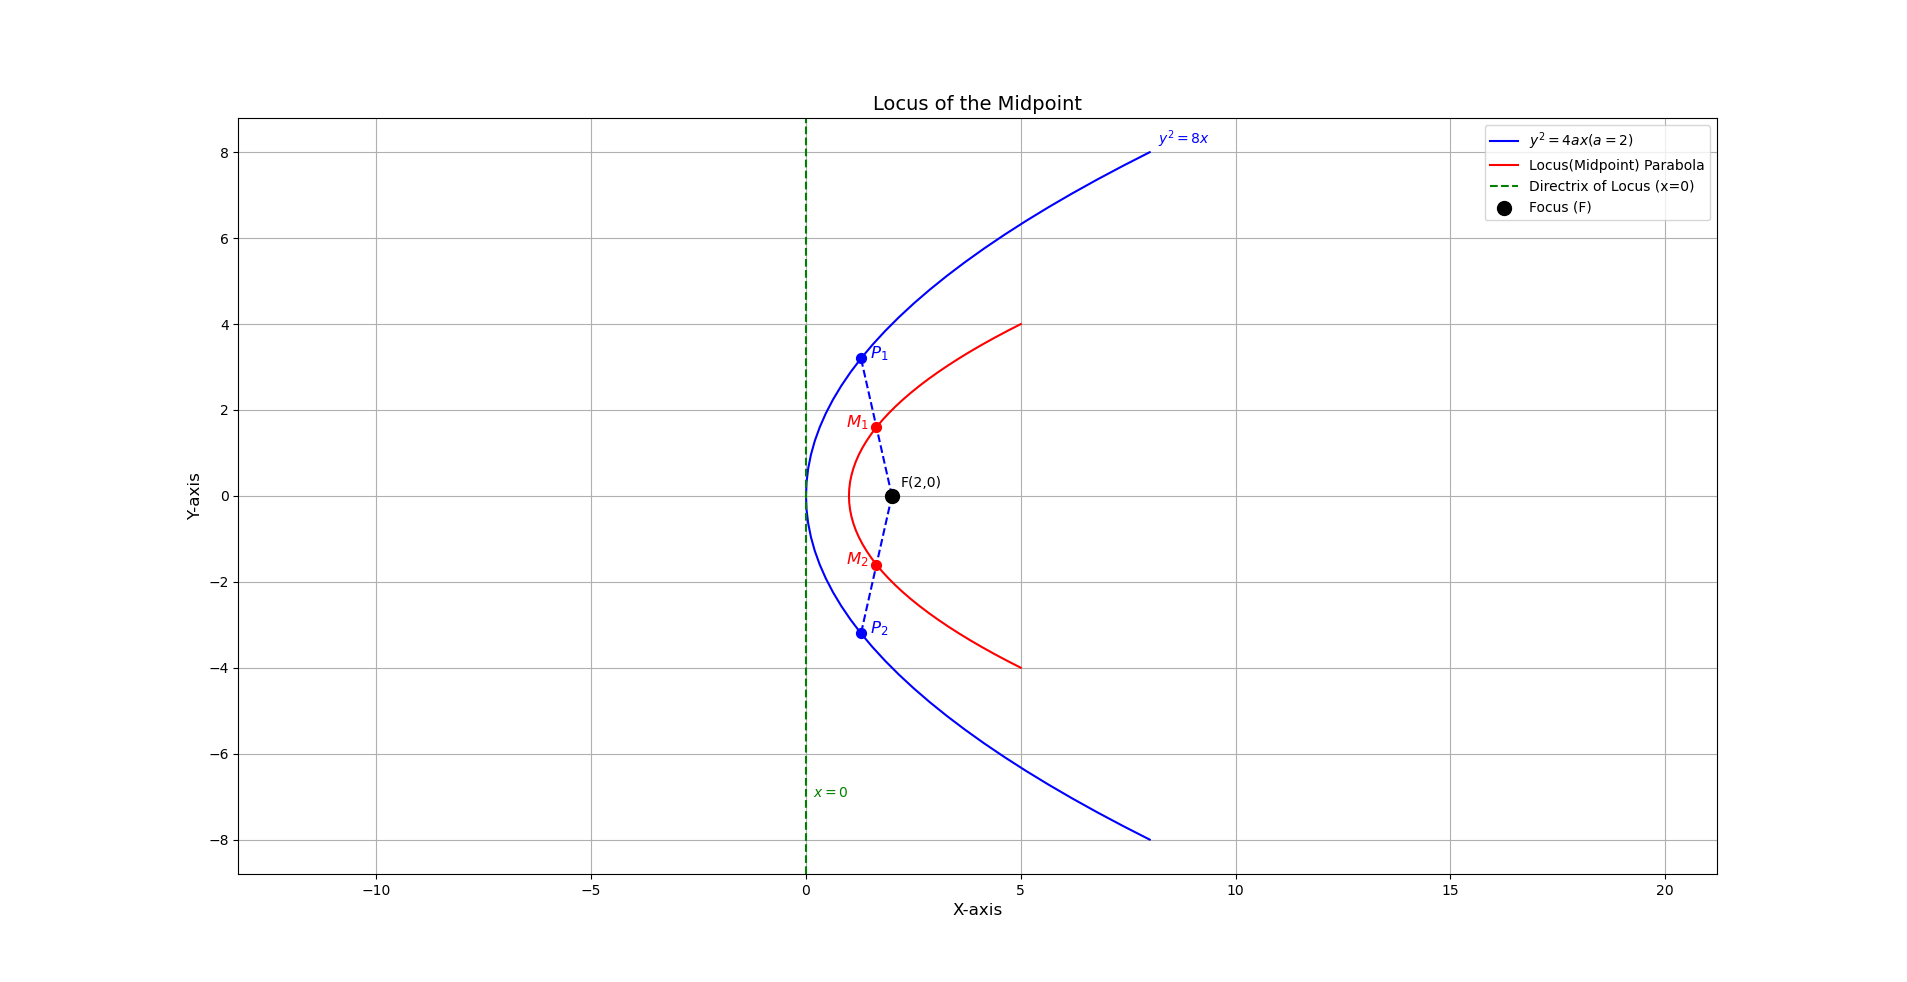
\includegraphics[width=0.98\columnwidth]{figs/fig1.png}
	\caption{}
   \label{}
\end{figure}
\end{document}  
